%!TEX root = ../prace.tex

\section{Plnička kyslíkových bomb}

Kyslíkové bomby je potřeba opětovně naplnit, pokud byl jejich obsah spotřebován. Stejně jako u Kyslíkové bomby, levým tlačítkem myši je možné rovnou doplnit zásoby kyslíku hráče. Pravým se pak otevře ovládací obrazovka.

\begin{figure}[!ht]\centering
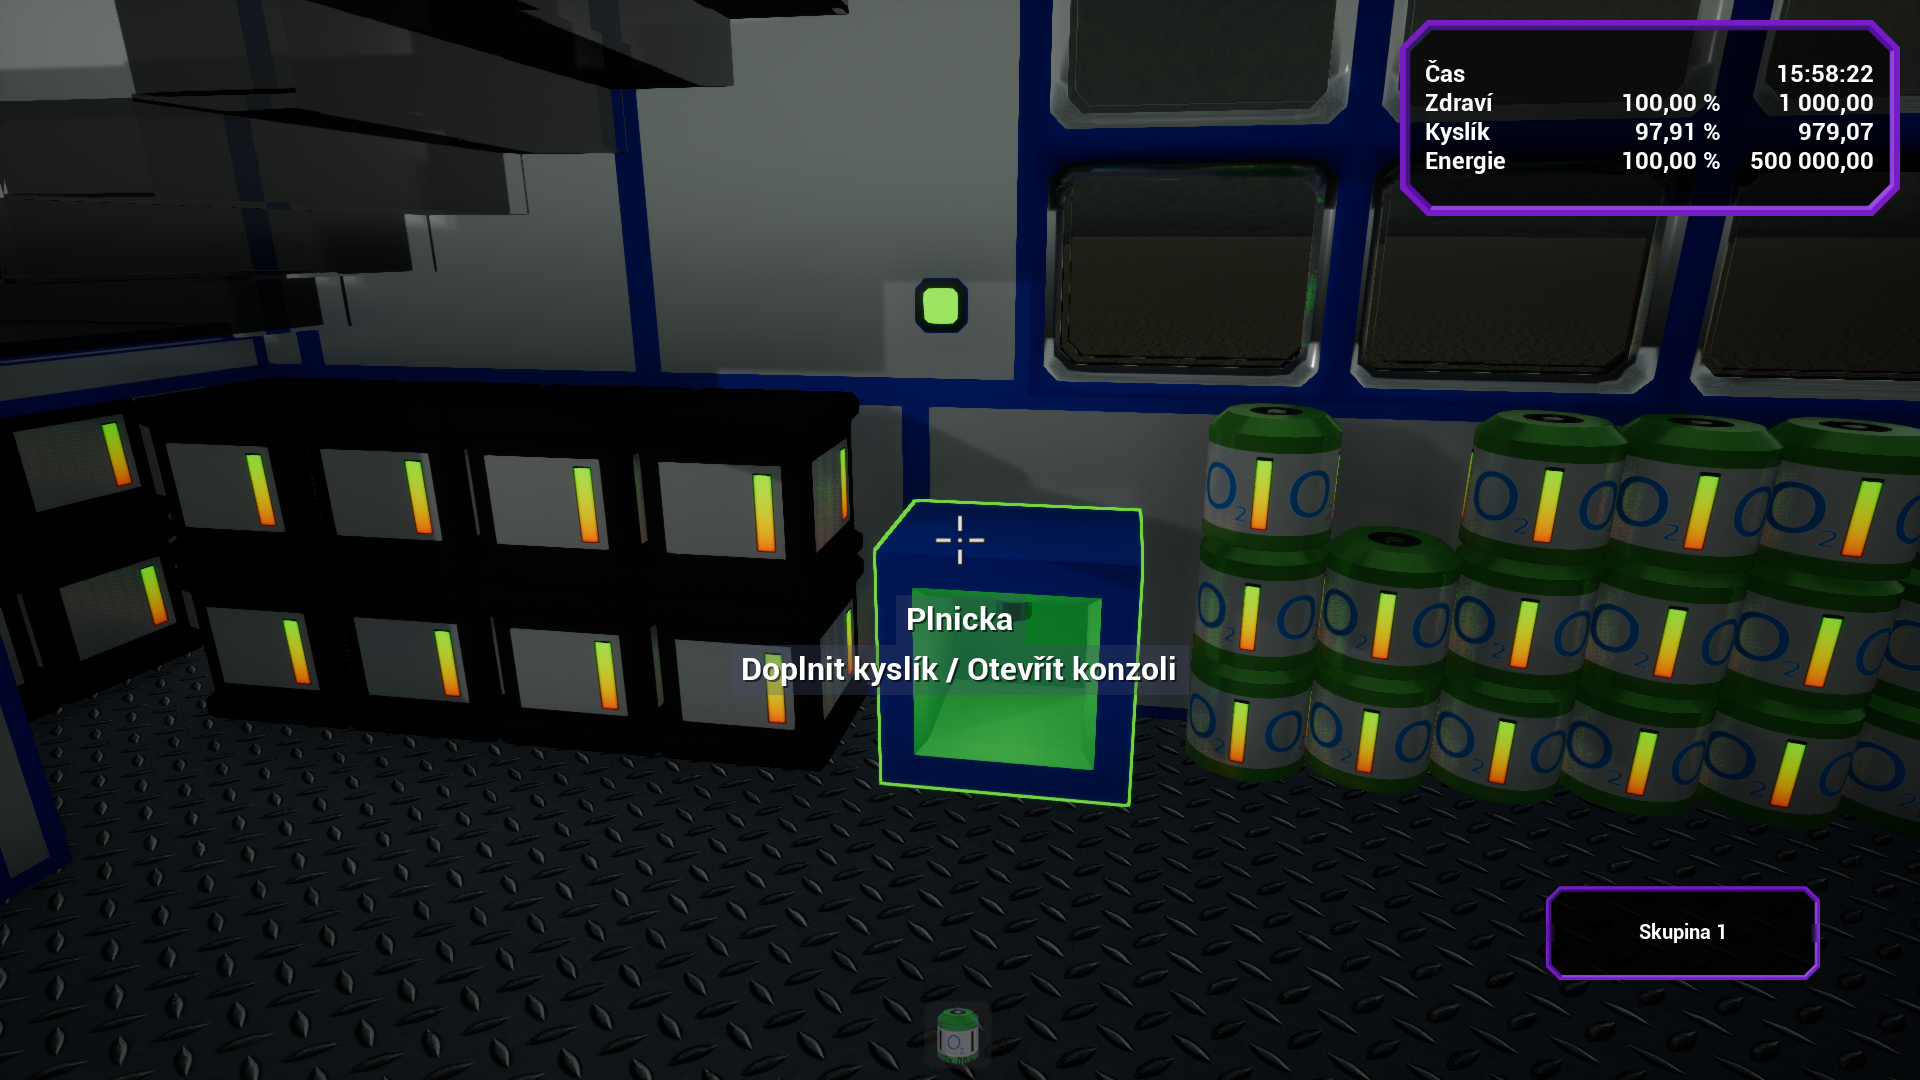
\includegraphics[ width=140mm]{../img/user/filler/0use}

\caption{Plnička kyslíkové bomby - náhled}
\label{fig:user_filler_0use}

\end{figure}

\FloatBarrier

Ta má v levé části přiřazený ovladač, případně je možné nejvýše jeden ovladač ze seznamu ovladačů přiřadit. Pokud je přiřazen ovladač, zapnutí bloku se řídí jeho nastavením. V pravé části je možné regulovat spotřebovávanou energii.

Uprostřed je možné vybrat bomby, které jsou v inventáři hráče, k naplnění.

\begin{figure}[!ht]\centering
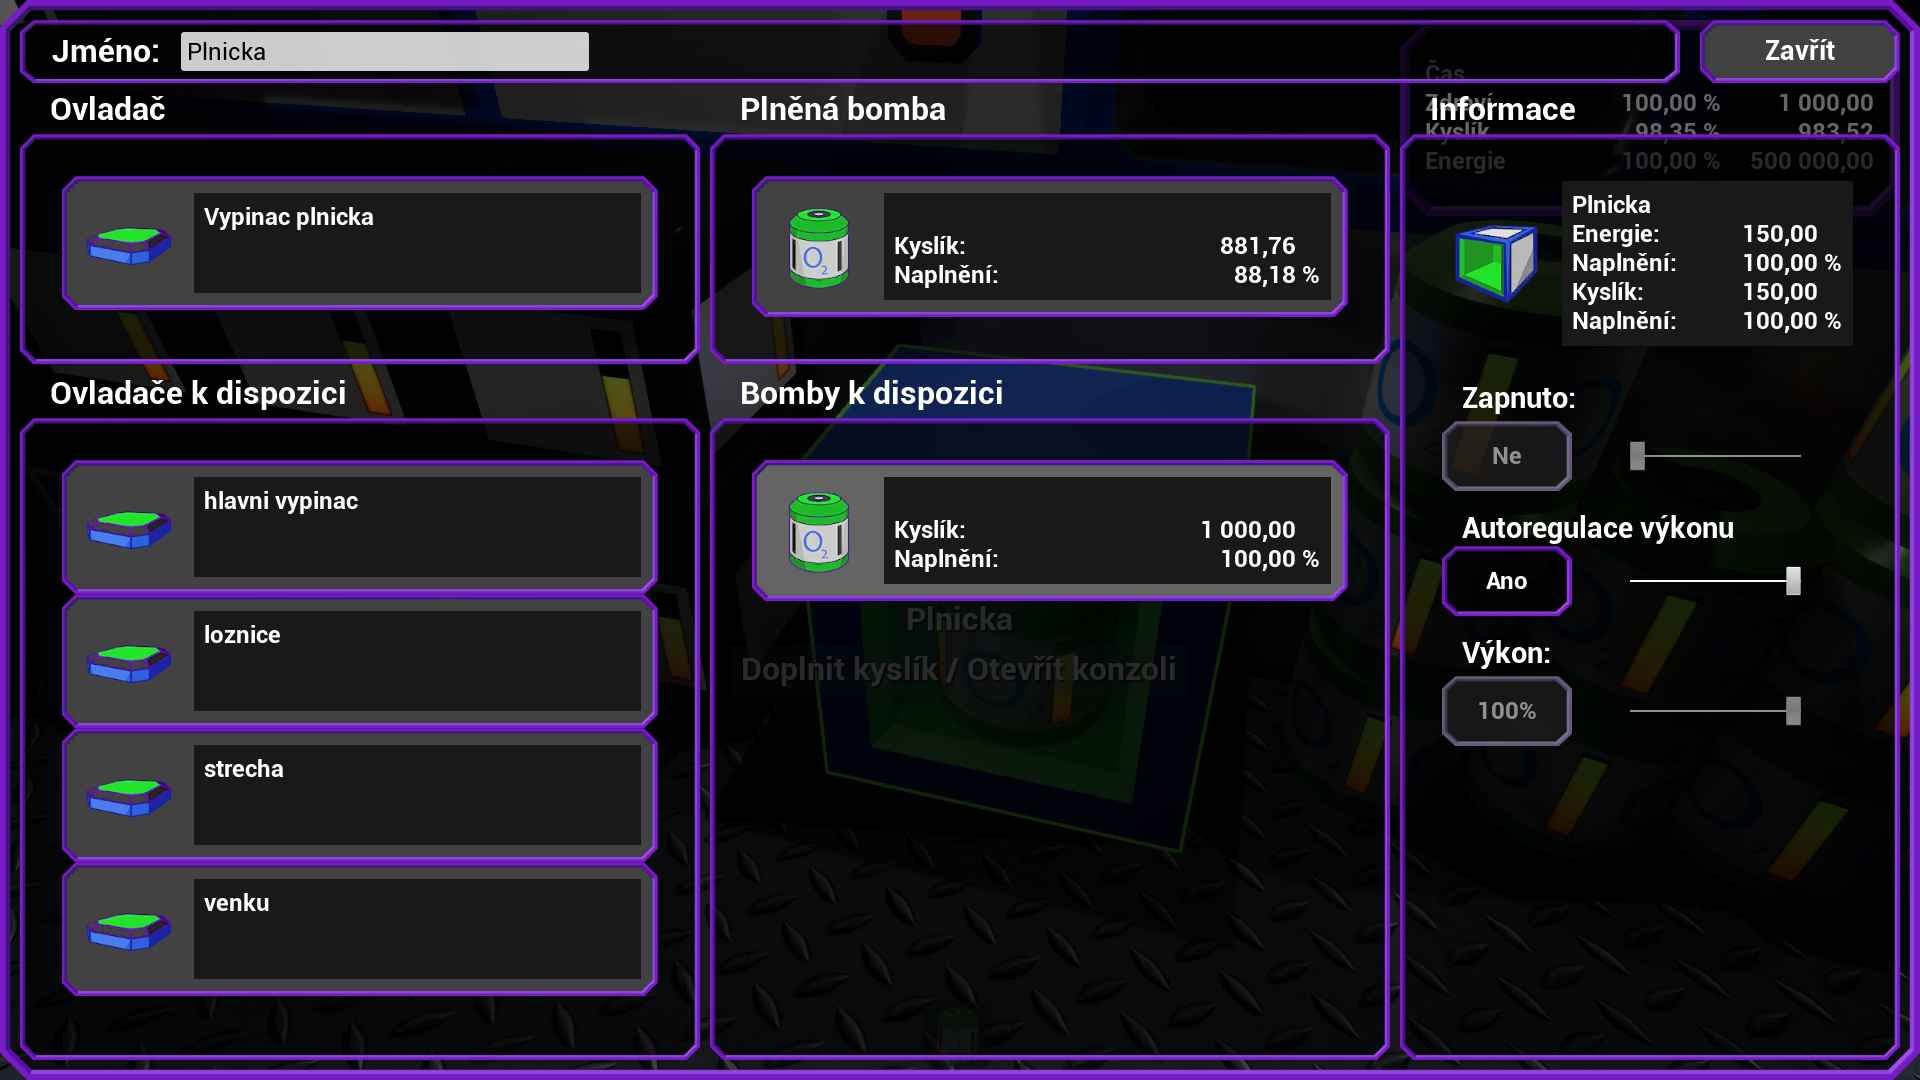
\includegraphics[ width=140mm]{../img/user/filler/1fill}

\caption{Plnička kyslíkové bomby - ovládací obrazovka}
\label{fig:user_filler_1fill}

\end{figure}

\FloatBarrier

Pokud je plnička zapnuta, generuje kyslík a ze své zásoby plní přiřazenou kyslíkovou bombu.

\begin{figure}[!ht]\centering
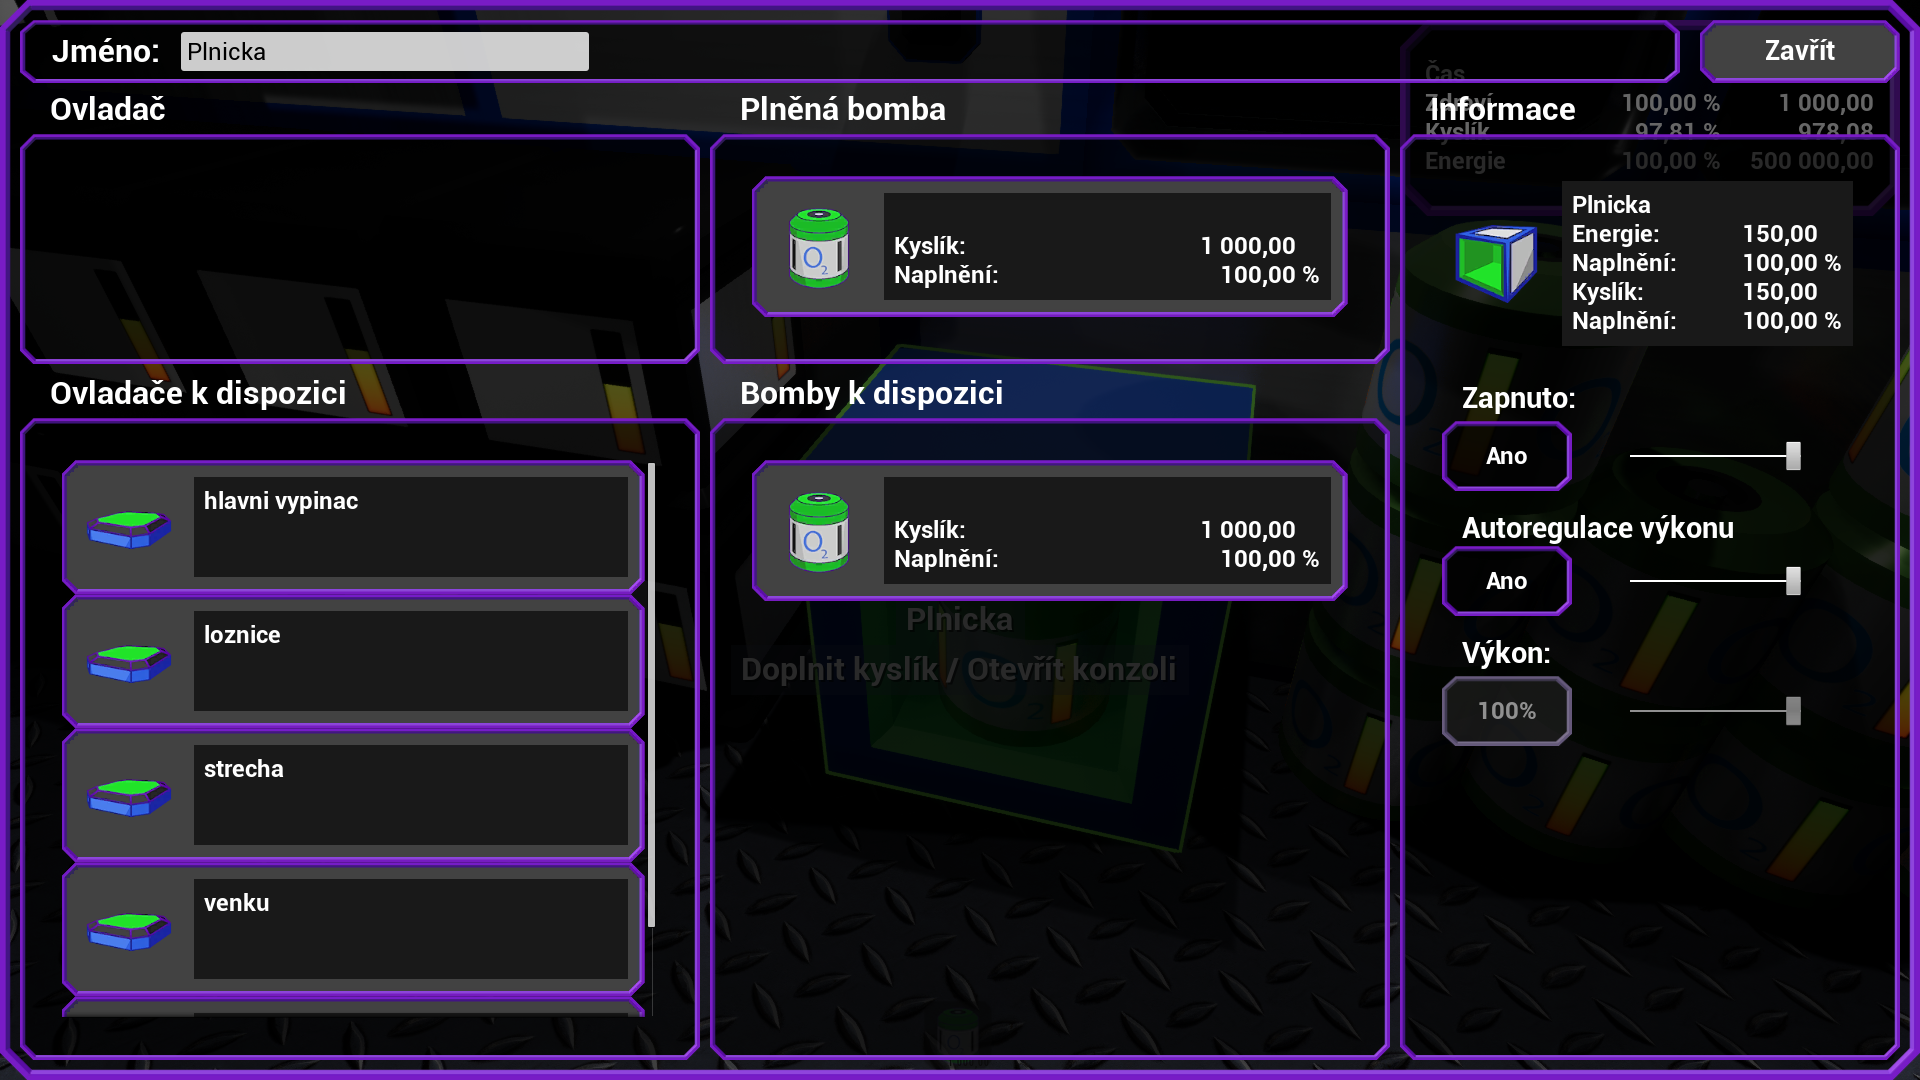
\includegraphics[ width=140mm]{../img/user/filler/2filled}

\caption{Plnička kyslíkové bomby - naplněno}
\label{fig:user_filler_2filled}

\end{figure}



\FloatBarrier